\documentclass[10pt,twocolumn,letterpaper]{article}

\usepackage{fullpage}
\usepackage{graphicx}

\author{David Simon}
\title{Task-Specific Filesystem Block Reorganization in Ext3}

\begin{document}

\maketitle

\begin{abstract}
Hard disk access times are the most significant performance bottleneck when
starting typical applications on contemporary personal computers and servers.
Most modern programs must load numerous libraries, resource files, modules, and
other pieces of information off disk before performing any useful work. Optimization
in this area should prove fruitful.

We attempted to reduce the amount of time consumed by hard disk activity during
the initialization of various programs. To do this, we observed which data blocks were
used during the initialization of various programs. Then, those blocks were moved
closer together, in the hope that the quantity and length of drive head seeks
would be reduced. The results were mixed; some applications received no particular
benefit from this optimiziation, while others were made to start significantly faster.
\end{abstract}

\section{Introduction}

Hard disk drives are, by a wide margin, the slowest internal storage devices commonly
used in modern computing. For a typical read or write, the disk head must first
\emph{seek} to the target block\cite{seektime}. On even the fastest hard disks\cite{deskstar}, one seek
can take several milliseconds, often orders of magnitude longer than the operation which will actually
use that data. Even if seeking is unnecessary because the disk head is already at the correct track, there is
often still a long delay waiting for the desired block to spin around to the head again\cite{latency}. When
many disk operations are required, tasks that would otherwise be immediately performing computations on data must first wait for these slow, mechanical processes to complete.

Ideally, to mitigate this problem, the next block to be requested should be physically near to
and after the current block\cite{autolocality}. When a seek or
spin wait is unavoidable, then it is better if the travel time required can at least be lessened by reducing the
physical distance between the current block and the next. The best scenario is when
as much disk time as possible is spent actually retreiving data, and as little as possible
wasted travelling from one request location to another.

It should be possible, with intelligent organization of data on the disk, to make the hard drive behave
more closely to this ideal.\texttt{Bolero}, the Block Organizer that Localizes Empirically-Related Objects, was developed as a proof-of-concept for this idea.

\section{Motivation for Bolero}\label{sec:motive}

In most filesystems, files are divided up
into one or more fixed-size chunks, called \texttt{blocks}CITETHIS. When a file's blocks
are not contiguous on disk, then the file is \texttt{fragmented}
and operations that require more than one block from the file are slow due to
seek and spin delays. The best proactive way to prevent fragmentation is to find contiguous
chunks of available space when allocating new files. Some older filesystems, such as FAT, were
very ineffective at doing this\cite{fathistory}.
FAT filesystems frequently had to be \texttt{defragmented} to maintain performance.
Modern filesystems, such as NTFS CITETHIS and ext3 CITETHIS, keep better track of free space,
and do not tend to fragment until the filesystem becomes nearly full. Advanced filesystems sometimes
use even more sophisticated strategies to prevent fragmentation, such as preallocating extra room to allow 
contiguous appending, or delaying physical allocation as long as possible so that better guesses
can be made about the characteristics of newly created files\cite{xfs}.

As important as these advancements have been, however, they do not address another, more subtle form of fragmentation: fragmentation between related files.
Just as slowdowns result when the various blocks of a file are distant from each other, when \emph{files} accessed in sequence are far from each other on the disk, significant unnecessary delays may result. For example, a large application such as an office suite or desktop environment requires numerous programs, shared libraries, icons, fonts, and other resources before it can start up completely. If these files must be read from disk but are spread apart from each other, the application's start-up time will increase.

The objective of Bolero is to reduce this type of fragmentation for that specific case, that of applications
starting up and loading a variety of resources from disk. It accomplishes this by moving data blocks that are typically accessed at about the same time closer together, and re-sequencing them into the order they are expected to be accessed.

\section{Filesystem Manipulation}

Because of the relative ease of extending and manipulating Linux filesystems and
kernel code, Bolero was be developed targetting Linux environments with ext3
filesystems. Ext3 is the standard filesystem used in Linux
environments, and is largely backwards compatible with ext2\cite{ext2journal}.
The general approach used by Bolero, however, is also applicable to most other commonly-used
filesystems.

The basic mechanism used by Bolero is the \texttt{libext2fs} library. This C
library, part of the standard \texttt{e2fstools} package, allows user-space programs
to open, scan, and make changes to ext2 filesystems. For Bolero, we wrote
a Python wrapper called \texttt{pyext2} around a subset of this library's functionality.
This library can open and scan through an ext2 or ext3 filesystem, report
various information about its contents, and swap the locations of arbitrary data
blocks while maintaining the filesystem's internal consistency.

Although there are some tentative mechanisms to allow the online rearrangement
of ext3 blocks\cite{ext3online}, Bolero is designed to run only on unmounted filesystems.
While it would be
convenient for the user to be able to manipulate a mounted filesystem, doing so
would add unnecessary complexity, making debugging and
development more difficult than necessary. Working with unmounted filesystems,
the reorganizer code can stay entirely in user-space, and does not have
to deal with the possibility of the file system's state being changed
midway through the process by other mechanisms outside its control.

With only the basic tool of swapping data blocks, a wide range of possible
defragmentation techniques are possible. Bolero includes \texttt{defragment.py}
a very simplistic proof-of-concept traditional defragmenter for ext3, which
simply reduces fragmentation within individual files. Because ext3 files do
not usually tend to fragment, the case for this kind of reorganization alone
is not very strong. However, individual file defragmentation is an important
basis for later, more sophisticated operations.

Once the reorganizer can reduce file discontiguity, it is possible to
use that same mechanism to reduce inter-file discontiguity, as explaiend
in section \ref{sec:motive}. Both types of defragmentation are necessary because the overall goal is to reduce the quantity of seeks and spin waits. The ideal state of affairs is for the disk to travel through
a sequence of files without interruption\cite{autolocality}, from the first block of the first file to the last
block of the last file with no delays or seeks.

FIXME MOVE PARAGRAPH BELOW ELSEWHERE.

There is one complication involved in attempting to make the blocks for
a given file contiguous. In ext3, data blocks are organized into larger
collections on disk called \texttt{block groups}\cite{ext2intro}. Each
block group contains both actual data blocks as well as \texttt{inodes},
which describe meta-data for each file. The headers and inode tables
for these groups create ``gaps'' of disk area which the defragmenter cannot
use to reduce discontiguity. The current implementation of Bolero ignores
this problem and simply skips over these gaps.

\section{Observing Disk Activity}

In order for the block reorganizer to decide what order is best for files
on disk, additional information is required.

FIXME ADD STUFF HERE ABOUT HOW OBSERVATION WORKS, WAS DEVELOPED, ETC.

To make development easier, Bolero will assume that it is observing (and
later reorganizing) the only filesystem on the disk. Future implementations of the
Bolero observer might attempt to correlate observations
made on several filesystems all simultaneously in use on the same disk, but
such a feature is outside the scope of this proposal. For now, Bolero will assume that
the information it records will reflect, as accurately as the OS can know,
all activity on the disk.

FIXME MOVE PARAGRAPH BELOW ELSEWHERE.

For example, many hard disks, upon discovering that a particular block has gone bad, will silently
remap that block to some other place on disk\cite{remapping}. This is a good thing for ensuring
data integrity, but it makes Bolero's optimization strategy more difficult, because
its idea of the ``physical'' disk location is actually still a level of abstraction away from
the actual disk. To overcome this, the observer can compare its recorded response
times with expected times, based on an understanding of how disks typically work.
If the delay in going from one seemingly ``contiguous'' block to the next
is unexpectedly long, then we may be able to assume that one of the blocks involved
has been silently remapped to some distant part of the disk. Such blocks can then be
assumed by the reorganizer to have poor contiguity regardless of proximity to other
blocks.

\section{Observation-Based Reorganization}

Once the observer is capable of producing useful information, that data then can be used
by the Bolero reorganizer to make informed decisions about file placement, justifying the
``Localizes Empirically-Related Objects'' part of the acronym. There are two
strategies for using this data: general optimization and task-specific optimization.

With general optimization, the reorganizer would use the recorded observations
to determine which files tend to be accessed within a short time from each
other, and in what order. It would then place files on disk in such a way as
to reduce average seek time and spin latency throughout the computer's operation.
Previous attempts at implementing this type of optimization at a
sub-filesystem level have resulted in significant performance benefits\cite{autolocality}.

The other approach, task-specific optimization, is simpler to
implement and may also (for its specific purpose) result in better performance. With this
approach, observations are limited to a particular, short-term task. For example,
the observer might start X and KDE, and record disk activity during its loading period,
up to the point at which it is ready for the user to begin working.
Within a short but disk-intensive period like this, even
though there will have been a lot of disk activity, any single file will
probably have been read from disk only once. The reorganizer can therefore simply
rearrange the relevant files on the disk to be contiguous and in the same order as that
recorded during the observational period, to reduce the amount of time taken for
that particular task. Previous efforts using this approach have been
successful in reducing large application startup times by over 60\%\cite{ala}.

FIXME REWRITE PARAGRPAH BELOW.

Because task-specific optimiziation is easier to implement and readily suggests
a metric, we chose it as the approach used by Bolero. However, since it is a
specialization of the general optimiziation approach, Bolero's success as
a proof-of-concept applies to both possible techniques.

\section{Measuring Results}

FIXME THIS ENTIRE SECTION SHOULD BE LARGELY REWRITTEN INTO THE ``OBSERVING DISK ACTIVITY'' SECTION.

In order to gauge how successful any optimization is, it is important to have
repeatable, objective measurements. A single benchmark would be insufficient to demonstrate
that Bolero is actually helpful in practical use. Although block reorganization has
potential benefits in many tasks, the most obvious one is the example presented above:
starting a large application. Therefore, during the process of developing Bolero, I will
also need to write a simple mechanism that can repeatedly start various large applications
and determine how beneficial Bolero's optimization strategies really are.

We tested the following applications:
\begin{itemize}
\item X Windows + KDE
\item OpenOffice
\item MySQL
\end{itemize}
Among these three applications, a wide range of shared libraries, subsystems, and user interface types
are involved. This helps to eliminate the influence of these factors on the final results;
ideally, the only factor being tested should be disk usage.

There are a number of difficulties that must be addressed to make these measurements useful.
The most important of these is the problem of determing when, exactly, the program has
``started up'' entirely. For some programs, this is fairly straightforward to define. For example,
Apache has started up entirely when it is able to respond to HTTP requests. Therefore,
to determine the start-up point for Apache, the measurement program merely has to act
as (or use) an HTTP client.

For GUI programs, however, the start-up point is more nebulously defined as when the user is
able to interact with the program. OpenOffice, for example, has started up completely when it is possible to open up and edit a document in it. Firefox has started up completely when it is capable of retrieving a web page. Testing these scenarios without actual human involvement will require application-specific solutions, such as
specially designed document macros or dynamic webpages that record the time at which they are loaded.

The situation for desktop environments, such KDE and GNOME, is even more complicated, since those are designed
to perform a wide range of disparate tasks. Such systems have not really started up \emph{entirely} until they are capable of performing every one of their varied functions. For example, it would not be enough to say that KDE has fully loaded when it is, say, possible to use its main menu to launch applications, because at that time KDE might still be busy loading other unrelated components, such as the background image manager, or the taskbar, or
the file management layer. It would be impractical to test each of these tasks individually,
so another method for finding the start-up point must be used.

One possible alternate way to find start-up times would be to monitor resource usage. All of the listed applications
above can be characterized by a busy loading period which, when finished, is followed by an idle period, where
the application waits for requests or user input to handle. The measurement program could monitor CPU usage and disk
activity to determine when this idle period begins. However, there are various factors which might prevent an application from ``loading'' entirely without user interaction; for example, if a shared library is required, it may only be partially loaded, with important but non-initialized code only being brought into memory when they are needed. For such situations, looking only at resource usage might result in misleadingly short times.

Concurrency presents another possible measurement hurdle. As mentioned above, the applications for
which start-up time would benefit the most from Bolero are those applications which involve a
large number of pieces, all potentially scattered around the filesystem. However, there is no guarantee
that these pieces will always be loaded in the same order by the application. KDE, for example, might reasonably start its window manager and its taskbar at the same time. Because of a certain amount of random
variation in the computer's state before and during the loading process, this might result in
slightly different disk access patterns for the same application. During one run, the taskbar might finish loading just before the window manager, while in another run, the opposite might be true. Multiple
measurements will be necessary to see how much the optimization helps despite this unpredictability.

One final issue that must be addressed for accurate measurement is the effect of caching. Both
the operating system and the drive itself will be, in light of the inherent slowness of hard drives,
doing a lot of caching. The operating system's cache can probably be manipulated directly; more
investigation into the Linux kernel will be required, but I suspect that clearing the software
cache may be as simple as unmounting and remounting the partition. The hard drive's internal cache
may be tricker to deal with, but one possible strategy might be to simply load several large chunks of
unused data from the drive, thereby filling the drive cache entirely or mostly (depending upon the mapping
and replacement schemes used) with garbage information that has nothing to do with the activities being tested.
The purpose of all of this cache-busting is to involve the actual hard drive as much as possible
in the tests, because Bolero's optimizations have to do with the physical limitations of hard drives. Although caching certainly helps programs to start up faster, it also interferes with my ability to test Bolero's actual effectiveness.

\section{Data Collected --- MySQL}

\begin{figure*}[!hbtp]
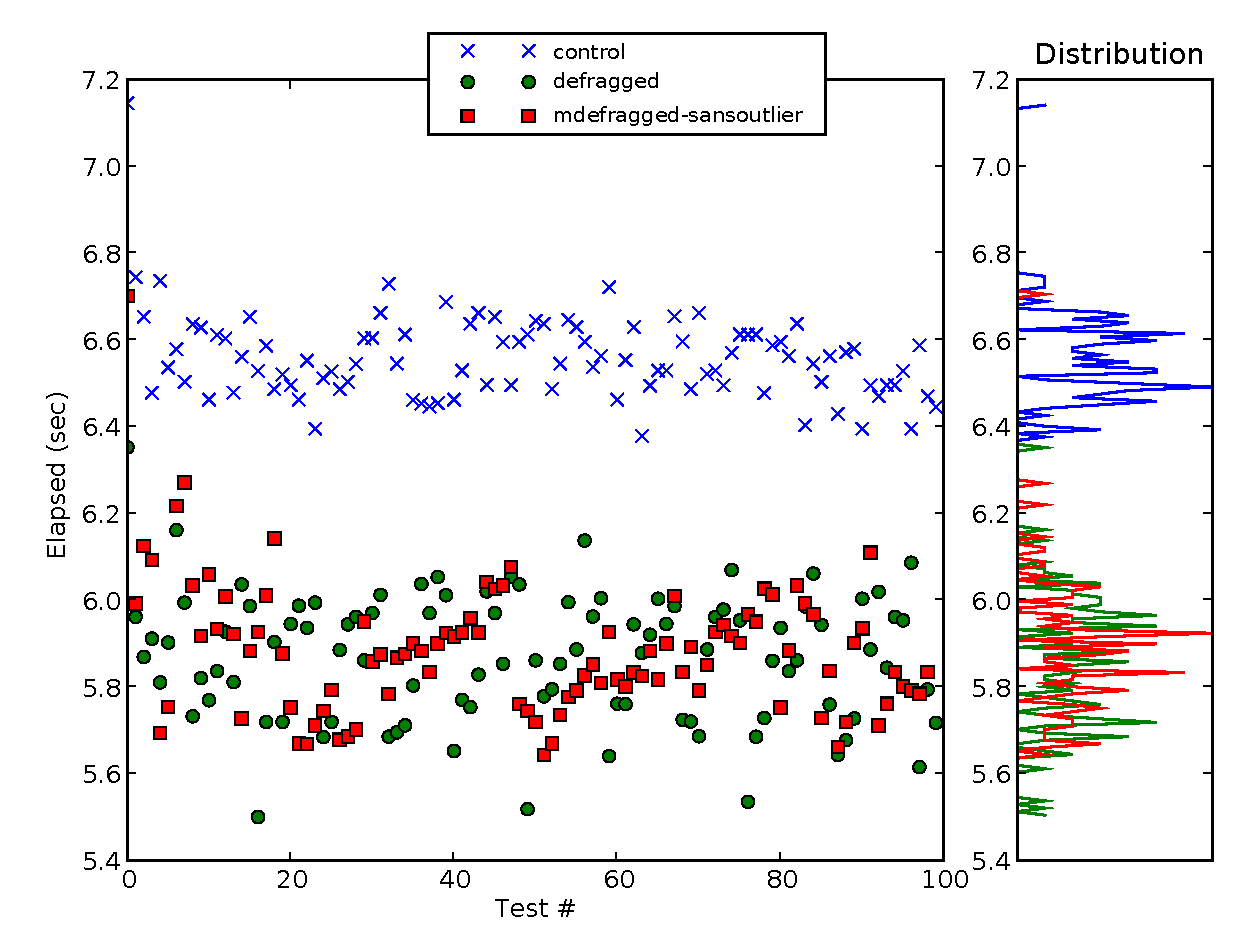
\includegraphics[scale=0.75]{mysql-chart.eps}
\caption{Start-up times for MySQL}
\label{mysqlchart}
\end{figure*}

tests/mysql/results/mysql-times-control (100 lines):  Mean=6558.43  StdDev=99.82
tests/mysql/results/mysql-times-control-frecord (100 lines):  Mean=6822.65  StdDev=98.09
tests/mysql/results/mysql-times-defragged (100 lines):  Mean=5873.32  StdDev=147.24
tests/mysql/results/mysql-times-mdefragged (100 lines):  Mean=5907.54  StdDev=279.13
tests/mysql/results/mysql-times-mdefragged-sansoutlier (99 lines):  Mean=5884.01  StdDev=152.76
Outlier in mdefragged: 8237

\section{Data Collected --- X \& KDE}

\begin{figure*}[!hbtp]
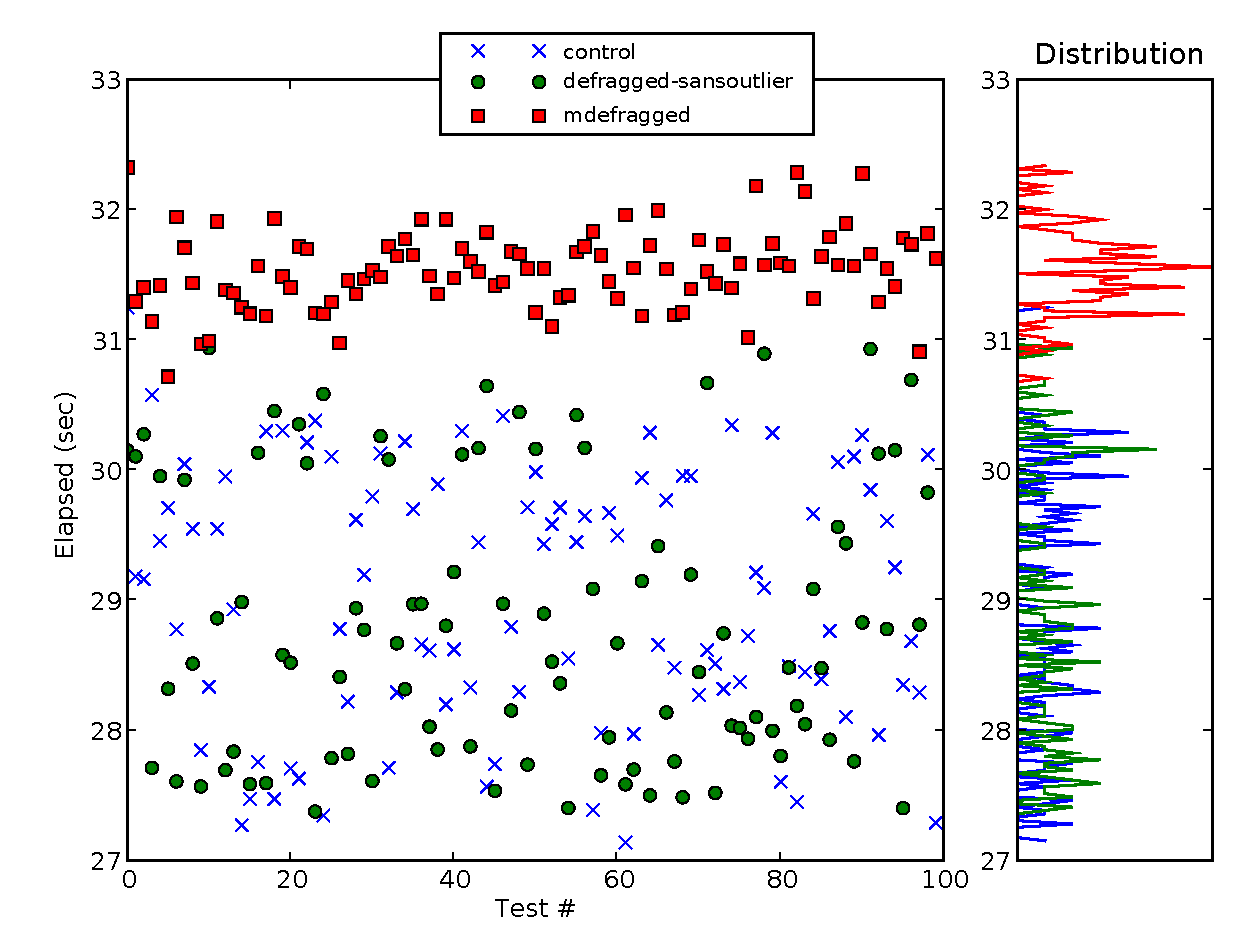
\includegraphics[scale=0.75]{kde4-chart.eps}
\caption{Start-up times for X and KDE4}
\label{kde4chart}
\end{figure*}

tests/kde4/results/kde4-times-control (100 lines):  Mean=29022.81  StdDev=972.04
tests/kde4/results/kde4-times-control-frecord (100 lines):  Mean=29833.02  StdDev=836.68
tests/kde4/results/kde4-times-defragged (100 lines):  Mean=29000.14  StdDev=2011.59
tests/kde4/results/kde4-times-defragged-sansoutlier (99 lines):  Mean=28827.84  StdDev=1057.64
tests/kde4/results/kde4-times-mdefragged (100 lines):  Mean=31543.05  StdDev=300.57
Outlier in defragged: 46058

\section{Data Collected --- OpenOffice}


\begin{figure*}[!hbtp]
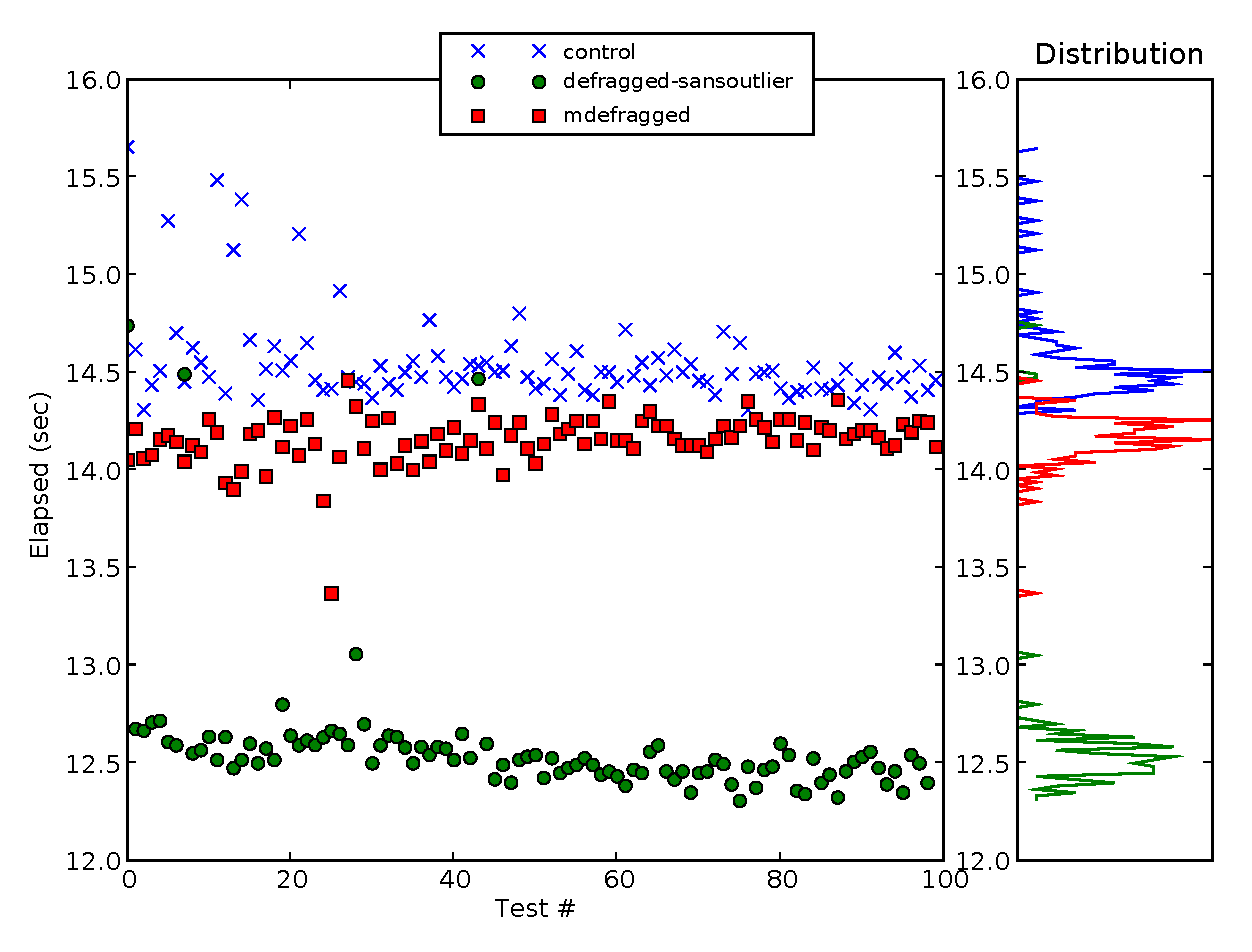
\includegraphics[scale=0.75]{openoffice-chart.eps}
\caption{Start-up times for OpenOffice}
\label{oochart}
\end{figure*}

tests/openoffice/results/openoffice-times-control (100 lines):  Mean=14551.48  StdDev=232.81
tests/openoffice/results/openoffice-times-control-frecord (100 lines):  Mean=14797.68  StdDev=148.20
tests/openoffice/results/openoffice-times-defragged (100 lines):  Mean=12780.42  StdDev=1954.91
tests/openoffice/results/openoffice-times-defragged-sansoutlier (99 lines):  Mean=12587.40  StdDev=367.09
tests/openoffice/results/openoffice-times-mdefragged (100 lines):  Mean=14157.44  StdDev=128.04
Outlier in defragged: 31889

\section{Analysis of Results}

\section{Possible Future Work}

\section{Conclusion}

Assuming that Bolero does end up being significantly useful, there are a number of directions that
the project could go in. A few of them are mentioned above: Bolero might be portable to other
operating systems or filesystems, or it might be possible to use it on more complicated multi-partition
or multi-disk setups. Additionally, there are probably other, more complex observation-based reorganization schemes
besides the two suggested above.

Before any of this is worth considering, though, the basic premise must first be tested. Can disk
blocks be reorganized based on observations of usage patterns to significantly improve performance?
There might be tremendous performance gains. Or, the unpredictability and complexity of modern
computers and applications may mean that careful organization of blocks in a seemingly helpful
sequence may really result in little to no perceivable benefit. The development of Bolero should conclusively
show which of these is the case.

FIXME NON-BREAKING LINES IN BIBLIOGRAPHY URLS ARE ANNOYING.

\bibliography{report}{}
\bibliographystyle{plain}

\end{document}
